\begin{problem}{1} ~\\
We can use XOR operation to ensure two nodes in the graph are in different set. There are two necessary conditions in order to reduce Bipartiteness to Formula-sat: for every edge $\{v,w\} \in E$, $v \in A$ and $w \in B$; for all edges of the graph the former condition should be fulfilled. \\
\\
We can use XOR operation of two nodes to implement the first condition, and AND operation of all edges to implement the second condition. Independent nodes can be in either Set A or Set B. It doesn't matter. So the variables representing independent nodes can be assigned either true or false.  For example, the following graph can be interpreted as this boolean formula: $(A \oplus B) \wedge (A \oplus C)$. A and B should be assigned different value to ensure the formula is true, so do A and C. If we take the variables that are assigned true to be Set A, and the variables that are assigned false to be Set B, then the formula is satisfiable if and only if the graph is bipartite. \\

\begin{figure}[H] 
\centering 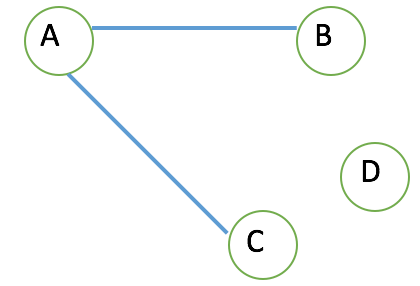
\includegraphics[width=0.4\columnwidth]{1_1}
\end{figure}

\end{problem}